%% PNAStmpl.tex
%% Template file to use for PNAS articles prepared in LaTeX
%% Version: Apr 14, 2008


%%%%%%%%%%%%%%%%%%%%%%%%%%%%%%
%% BASIC CLASS FILE
%% PNAStwo for two column articles is called by default.
%% Uncomment PNASone for single column articles. One column class
%% and style files are available upon request from pnas@nas.edu.
%% (uncomment means get rid of the '%' in front of the command)

%\documentclass{pnasone}
\documentclass{pnastwo}

%%%%%%%%%%%%%%%%%%%%%%%%%%%%%%
%% Changing position of text on physical page:
%% Since not all printers position
%% the printed page in the same place on the physical page,
%% you can change the position yourself here, if you need to:

% \advance\voffset -.5in % Minus dimension will raise the printed page on the
                         %  physical page; positive dimension will lower it.

%% You may set the dimension to the size that you need.

%%%%%%%%%%%%%%%%%%%%%%%%%%%%%%
%% OPTIONAL GRAPHICS STYLE FILE

%% Requires graphics style file (graphicx.sty), used for inserting
%% .eps files into LaTeX articles.
%% Note that inclusion of .eps files is for your reference only;
%% when submitting to PNAS please submit figures separately.

%% Type into the square brackets the name of the driver program
%% that you are using. If you don't know, try dvips, which is the
%% most common PC driver, or textures for the Mac. These are the options:

% [dvips], [xdvi], [dvipdf], [dvipdfm], [dvipdfmx], [pdftex], [dvipsone],
% [dviwindo], [emtex], [dviwin], [pctexps], [pctexwin], [pctexhp], [pctex32],
% [truetex], [tcidvi], [vtex], [oztex], [textures], [xetex]

%\usepackage[dvips]{graphicx}

%%%%%%%%%%%%%%%%%%%%%%%%%%%%%%
%% OPTIONAL POSTSCRIPT FONT FILES

%% PostScript font files: You may need to edit the PNASoneF.sty
%% or PNAStwoF.sty file to make the font names match those on your system.
%% Alternatively, you can leave the font style file commands commented out
%% and typeset your article using the default Computer Modern
%% fonts (recommended). If accepted, your article will be typeset
%% at PNAS using PostScript fonts.

% Choose PNASoneF for one column; PNAStwoF for two column:
%\usepackage{PNASoneF}
\usepackage{PNAStwoF}

%%%%%%%%%%%%%%%%%%%%%%%%%%%%%%
%% ADDITIONAL OPTIONAL STYLE FILES

%% The AMS math files are commonly used to gain access to useful features
%% like extended math fonts and math commands.

\usepackage{amssymb,amsfonts,amsmath}

%\usepackage{subcaption}
\graphicspath{ {paper_figures2/} }

\usepackage{tikz}

%\usepackage{sansmath}

%\usepackage[font={sf, small}]{caption}

%%%%%%%%%%%%%%%%%%%%%%%%%%%%%%
%% OPTIONAL MACRO FILES
%% Insert self-defined macros here.
%% \newcommand definitions are recommended; \def definitions are supported

%\newcommand{\mfrac}[2]{\frac{\displaystyle #1}{\displaystyle #2}}
%\def\s{\sigma}

%\DeclareMathSizes{9}{8}{7}{7}

%\DeclareMathOperator*{\argmin}{arg\,min}

\newcommand{\SI}[0]{{\it SI Materials and Methods}}
\newcommand{\fig}[0]{Fig.}


\makeatletter
\newcommand{\customlabel}[2]{%
\protected@write \@auxout {}{\string \newlabel {#1}{{#2}{}}}}
\makeatother

\customlabel{fig:DV_view}{S1}
\customlabel{fig:membrane_curve}{S2}
\customlabel{fig:raw_data3}{S3}
\customlabel{fig:1d_example}{S4}
\customlabel{fig:spheres}{S5}
\customlabel{fig:eigenvalues}{S6}
\customlabel{fig:PCA_data1}{S7}
\customlabel{fig:PCA_data2}{S8}

%%%%%%%%%%%%%%%%%%%%%%%%%%%%%%
%% Don't type in anything in the following section:
%%%%%%%%%%%%
%% For PNAS Only:
\contributor{Submitted to Proceedings
of the National Academy of Sciences of the United States of America}
\url{www.pnas.org/cgi/doi/10.1073/pnas.0709640104}
\copyrightyear{2008}
\issuedate{Issue Date}
\volume{Volume}
\issuenumber{Issue Number}
%%%%%%%%%%%%

\begin{document}

%%%%%%%%%%%%%%%%%%%%%%%%%%%%%%


%% For titles, only capitalize the first letter
%% \title{Almost sharp fronts for the surface quasi-geostrophic equation}

\title{Temporal ordering and registration of images in studies of developmental dynamics}

%% Enter authors via the \author command.
%% Use \affil to define affiliations.
%% (Leave no spaces between author name and \affil command)

%% Note that the \thanks{} command has been disabled in favor of
%% a generic, reserved space for PNAS publication footnotes.

%% \author{<author name>
%% \affil{<number>}{<Institution>}} One number for each institution.
%% The same number should be used for authors that
%% are affiliated with the same institution, after the first time
%% only the number is needed, ie, \affil{number}{text}, \affil{number}{}
%% Then, before last author ...
%% \and
%% \author{<author name>
%% \affil{<number>}{}}

%% For example, assuming Garcia and Sonnery are both affiliated with
%% Universidad de Murcia:
%% \author{Roberta Graff\affil{1}{University of Cambridge, Cambridge,
%% United Kingdom},
%% Javier de Ruiz Garcia\affil{2}{Universidad de Murcia, Bioquimica y Biologia
%% Molecular, Murcia, Spain}, \and Franklin Sonnery\affil{2}{}}

\author{Carmeline~J.~Dsilva\affil{1}{Department of Chemical and Biological Engineering, Princeton University, Princeton, New Jersey, USA},
Bomyi~Lim\affil{1}{},
Thomas~J.~Levario\affil{2}{School of Chemical and Biomolecular Engineering, Georgia Institute of Technology, Atlanta, Georgia, USA},
Hang~Lu\affil{2}{},
Amit~Singer\affil{3}{Department of Mathematics, Princeton University, Princeton, New Jersey, USA} \affil{4}{Program in Applied and Computational Mathematics, Princeton University, Princeton, New Jersey, USA},
Stanislav~Y.~Shvartsman\affil{1}{} \affil{5}{Lewis-Sigler Institute for Integrative Genomics, Princeton University, Princeton, New Jersey, USA},
\and
Ioannis~G.~Kevrekidis\affil{1}{} \affil{4}{Program in Applied and Computational Mathematics, Princeton University, Princeton, New Jersey, USA}}

\contributor{Submitted to Proceedings of the National Academy of Sciences
of the United States of America}

\significancetext{Cross-sectional imaging studies are commonly used to study developmental dynamics in multiple organisms. 
%
In these studies, a representative developmental trajectory is reconstructed from snapshots of different embryos, each of which has been arrested at a different point of its development. 
%
One of the first steps in this reconstruction involves registration and temporal ordering of images. 
%
Here we show that both of these tasks can be automated and combined in a single step using recent advances in data mining. 
%
To illustrate this approach, we temporally order and register several datasets collected in cross-sectional studies of cell signaling in the early fruit fly embryo.}

%% The \maketitle command is necessary to build the title page.
\maketitle

%%%%%%%%%%%%%%%%%%%%%%%%%%%%%%%%%%%%%%%%%%%%%%%%%%%%%%%%%%%%%%%%
\begin{article}

\begin{abstract}

Imaging studies provide unique insights into the dynamics of developmental processes. 
%
A large number of imaging studies are based on a cross-sectional experimental design, where developmental progress is arrested in a population of embryos, each of which is at a different point along its developmental trajectory. 
%
The goal is then to temporally order the data to reconstruct representative developmental dynamics from snapshots provided by the collection of embryos.
%
Images of different biological samples must first be registered before they can be temporally ordered.
%
When such data sets are large, noisy, and/or if the developmental changes are subtle, these tasks can be difficult to perform manually.
%
We present an automated approach to simultaneously register and temporally order data from such cross-sectional studies.
%
The approach is based on vector diffusion maps, a broadly applicable manifold learning technique that does not require {\it a priori} knowledge of image features or a parametric model of the developmental dynamics.
%
%Furthermore, these techniques can separate multiple trajectories within the same data set.
%
We use this method to extract developmental dynamics from collections of images from a cross-sectional study of cell signaling during dorsoventral patterning of the {\it Drosophila} embryo.
\end{abstract}


%% When adding keywords, separate each term with a straight line: |
\keywords{temporal ordering | image registration | vector diffusion maps}

%% Optional for entering abbreviations, separate the abbreviation from
%% its definition with a comma, separate each pair with a semicolon:
%% for example:
%% \abbreviations{SAM, self-assembled monolayer; OTS,
%% octadecyltrichlorosilane}

% \abbreviations{}

%% The first letter of the article should be drop cap: \dropcap{}
%\dropcap{I}n this article we study the evolution of ''almost-sharp'' fronts

%% Enter the text of your article beginning here and ending before
%% \begin{acknowledgements}
%% Section head commands for your reference:
%% \section{}
%% \subsection{}
%% \subsubsection{}



\dropcap{E}xperimental studies of developmental dynamics fall in two broadly defined categories: longitudinal and cross-sectional \cite{diggle2002analysis}.
%
In longitudinal studies, developmental progress is monitored over time in the same embryo \cite{roelens2013live, keller2013imaging}.
%
In a cross-sectional study, developmental dynamics is reconstructed from multiple embryos, each of which contributes only a snapshot of a chemical or morphological process along its developmental trajectory \cite{jaeger2004dynamic, fowlkes2008quantitative}.
%
Here we focus on cross-sectional studies, which have a time-honored history and still present the only option for most organisms.
%
In a typical cross-sectional study, a group of embryos is fixed using a procedure that arrests their development and stained with chemicals that visualize a handful of cellular processes.
%
Fixed embryos are then imaged using any given number of microscopy techniques.
%
%Recent advances in physical manipulation and imaging of embryos produce rapidly increasing volumes of cross-sectional data, in which every embryo is observed at a different developmental time point and at a different geometric orientation.
%
Importantly, the ``age'' of any given embryo arrested in its development is not quantitatively known; typically what is known is
a certain time window to which a collection of embryos belongs \cite{ng2012large, richardson2014emage, castro2009automatic}.
%to high accuracy.
%
In order to recover the developmental dynamics from such data sets, snapshots of different embryos must first be spatially aligned or {\em registered} to factor out the relevant geometric symmetries (e.g., translations and rotations), and then ordered in time.
%
We show how recently developed dimensionality reduction algorithms can automate {\it and combine} both of these tasks.

Temporal ordering and registration of images can be done manually
when the number of images is small and the differences between them are visually apparent. 
%
\fig~\ref{fig:fish} shows a caricature of fish development which illustrates the processes of growth and patterning.
%
In this case, temporal ordering can be accomplished by arranging the fish by size, which is monotonic with the developmental progress.
%
Image registration is based on obvious morphological landmarks, such as the position of head and fins.
%
In contrast to this example, real data poses nontrivial challenges for both registration and temporal ordering.
%
In general, the landmarks needed for registration (here, the heads and fins) as well as the attributes which can be used to order the data (such as the body length) are not known {\it a priori}.
%
Additional challenges arise from embryo-to-embryo variability, sample size, and measurement noise.

\begin{figure}[t]
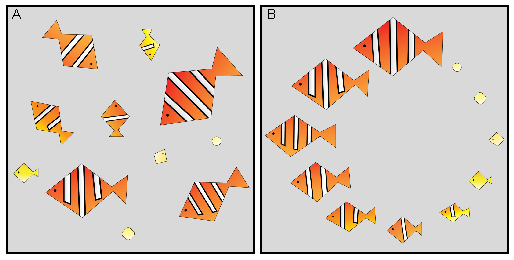
\includegraphics[width=8.7cm]{fig1}
\caption{Caricature illustrating the tasks of image registration and temporal ordering. {\xfigtextfontit (A)} Images of ``samples'', each in a different orientation and a different stage of development. {\xfigtextfontit (B)} Registered and ordered samples. For this caricature, the registration and ordering is straightforward because the data set is small and the developmental changes are easy to recognize visually.}
%\label{fig:fish}
\customlabel{fig:fish}{1}
\customlabel{subfig:fish_unordered}{\ref{fig:fish}{\it A}}
\customlabel{subfig:fish_ordered}{\ref{fig:fish}{\it B}}
\end{figure}

%%%YGK put an arrow in the disc

Image registration has been studied in a variety of contexts \cite{zitova2003image, rowley1998rotation, hajnal2010medical, greenspan1994rotation, zhao2003face}, 
and most registration algorithms are based on landmarks, such as the head and fins in \fig~\ref{fig:fish}.
%
In contrast, our approach requires no such information. 
%
It is based on a manifold learning algorithm (vector diffusion maps, VDM \cite{singer2012vector}) which simultaneously addresses the problems of registration and temporal ordering. 
%
This algorithm is one of several influential nonlinear dimensionality reduction techniques that have been developed over the past decade \cite{Belkin2003, coifman2005geometric, coifman2006geometric, tenenbaum2000global, roweis2000nonlinear}. 
%
The technique has been used for data mining in
applications ranging from analysis of cryo-electron microscopy (cryo-EM) images of individual molecules to face recognition, and is sufficiently general to be applicable to a wide variety of biological imaging studies. 
%
Here the algorithm is adapted for simultaneous registration and temporal ordering of images from cross-sectional studies of developmental dynamics, with the main objective of revealing stereotypic developmental trajectories.
%
To illustrate our approach, we analyze three data sets from a study of {\it Drosophila} embryogenesis, one of the best experimental models for studies of developmental dynamics \cite{jaeger2012drosophila}.
%
%The first data set, shown in Figure~\ref{subfig:raw_data1}, is relatively simple and will allow us to both illustrate and validate this approach.
%
%In the second data set, shown in Figure~\ref{subfig:raw_data2}, the dynamics are significantly more complex.
%
%Here, we will show that we can recover a trajectory that is qualitatively consistent with current knowledge.
%
%The third set consists of data collected from both wild type and mutant embryos, where joint processing of the data will help to visualize the different sources of variability along distinct developmental paths.

%\begin{itemize}
%\item Imaging data is becoming increasingly prevalent in biology research.
%
%\item General motivation about biology data ...
%
%\item Need methods to organize data, visualize, ...
%
%\item REDUCTION is important, reduction because of symmetry and reduction because of content
%
%\item There are a bunch of recent techniques- some established (like dmaps), some very fresh, like synchronization or VDMaps,  that have had their own reasons to be developed but they are as if tailor made for what we would want to do
%\end{itemize}


\section{Results}

\subsection{Vector diffusion maps for registration and temporal ordering}

%%%YGK  when I read this I think of Eiffel tower pictures, not of ours - there is a transition... careful where we do it.
%
%Our goal is to organize data sets from cross-sectional studies of developmental processes in a meaningful and informative way.
%
%We will show that dimensionality reduction algorithms can simultaneously register and temporally order the images to give us a meaningful picture of the underlying developmental dynamics.
%
Our approach is based on vector diffusion maps \cite{singer2012vector}, a manifold learning
technique developed for data sets which contain two types of sources of variability:
geometric symmetries (such as translations and rotations of the images due to the experimental setup) which one would like to factor out,
and ``additional" directions of variability (such as temporal dynamics) which one wants to uncover.
%
Vector diffusion maps combine two algorithms, {\em angular synchronization} \cite{singer2011angular} for image registration and {\em diffusion maps} \cite{coifman2005geometric} for extracting intrinsic low-dimensional structure in data, into a single computation that allows us to simultaneously register and temporally order our images.
%
%Vector diffusion maps has been used to classify images from cryo-electron microscopy (cryo-EM) experiments, where each image is a projection of a randomly oriented molecule.
%
%%%YGK to imply which rotations we need to have discussed it above
%%
We will use the algorithm to register images of {\it Drosophila} embryos with respect to rotations and translations, as well as uncover the main direction of variability {\it after} removing translational and rotational symmetries.
%
We assume that, in these sets of images, the main direction of variability is parameterized by the developmental time of each embryo, so that uncovering this direction will allow us to recover the developmental dynamics.

%%%somewhere I want a sentence that says this is for general symmetry groups of some kind, and HERE it is for..... (maybe in SI)
Angular synchronization uses pairwise alignment information to register a set of images in a globally consistent way.
%
A schematic illustration of angular synchronization is shown in \fig~\ref{subfig:synch1}, where each image is represented as a vector, and the goal is to align the set of vectors.
%
We first compute the angles needed to align pairs of vectors (or images).  
%
In general, this requires no template function \cite{ahuja2007template} or image landmarks \cite{ian1998statistical}.
%
Using the alignment angles between all pairs of vectors, angular synchronization finds the set of rotation angles (one angle for each vector) that is most consistent with {\it all} pairwise measurements (see {\it SI Materials and Methods}); this is illustrated in \fig~\ref{subfig:synch2}.
%
In this schematic, registration via angular synchronization is trivial, as the pairwise measurements contain no noise.
%
However, the algorithm can successfully register data sets even when many of the pairwise measurements are inaccurate \cite{singer2011angular}.
%

%
After removing variability due to translations and rotations, the developmental dynamics may be revealed by ordering the data along the one-dimensional manifold that parameterizes most of the remaining variability in the data.
%%%
%%%YGK feels like repeats
%%%
%
Such a manifold can be discovered using diffusion maps \cite{coifman2005geometric}, a nonlinear dimensionality reduction technique that uncovers an intrinsic parametrization of data that lies on a low-dimensional, perhaps nonlinear, manifold in high-dimensional space.
%
The idea is illustrated in \fig~\ref{subfig:dmaps1}, where the data are two-dimensional points which lie on a one-dimensional nonlinear curve.
%
We use {\it local} information about the data to find a parametrization  which respects the underlying manifold geometry: we want points which are close in high-dimensional space (e.g., images which look similar) to be close in our parametrization.
%
This idea of locality is denoted by the edges in \fig~\ref{subfig:dmaps1}.
%
Data points which are close are connected by dark edges, and clearly, the dark edges are more ``informative" about the low-dimensional structure of the data.
%
The color in \fig~\ref{subfig:dmaps2} depicts the one-dimensional parametrization or ordering of the data that we can detect visually.
%
In our working examples, each data point will be much higher dimensional (e.g., a pixelated image), and so we cannot extract this low-dimensional structure visually.
%
Instead, we will use diffusion maps to automatically uncover a parametrization of our high-dimensional data (see \SI).
%
Diffusion maps generalizes directly from one-dimensional nonlinear curves to higher-dimensional manifolds.
%
Thus, when our experiments have additional sources of variability (such as distinct populations of embryos) in addition to developmental dynamics, diffusion maps can provide an informative organization of our data which highlights both of these variability sources.
%We will assume that our data are approximately one-dimensional, and that this dimension is parameterized by time, such that ordering our data along this main dimension/direction will temporally order our data.

Both angular synchronization and diffusion maps use pairwise information to uncover global structure in the data.
%
Angular synchronization uses pairwise alignment information to find translations and rotations which are globally consistent, and diffusion maps uses pairwise distances to find global parametrizations which are (geometrically) informative.
%
Vector diffusion maps combines both steps into a single computation (see \SI), simultaneously addressing the tasks of registration and temporal ordering.
%
%The algorithm uses information about pairwise alignments {\em and} pairwise distances to find a global parametrization of the data, while registering images which are ``close'' .
%
%It is thus perfectly suited for our task of registering and temporally ordering cross-sectional imaging data.
%

\begin{figure}[t]
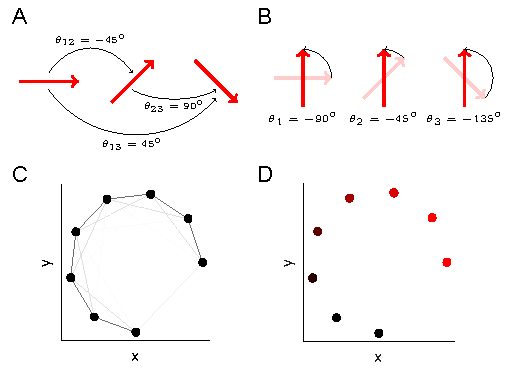
\includegraphics[width=8.7cm]{fig2}
\caption{Schematic illustrating angular synchronization and diffusion maps. {\xfigtextfontit (A)} Set of vectors, each in a different orientation. The pairwise alignment angles are indicated. {\xfigtextfontit (B)} The vectors from {\xfigtextfontit A}, each rotated about their midpoint so that the set is globally aligned. Note that the chosen rotation angles are consistent with the pairwise alignments in {\xfigtextfontit A}: the differences between a pair of angles in {\xfigtextfontit B} is the same as the pairwise angle in {\xfigtextfontit A}. {\xfigtextfontit (C)} Data points (in black) which lie on a one-dimensional nonlinear curve in two dimensions. Each pair of points is connected by an edge, and the edge weight is related to the Euclidean distance between the points through the diffusion kernel (see {\xfigtextfontit \SI}), so that close data points are connected by darker (``stronger'') edges. {\xfigtextfontit (D)} The data in {\xfigtextfontit C}, colored by the first (non-trivial) eigenvector from the diffusion map computational procedure. The color intensity is monotonic with the perceived curve arclength, thus parameterizing the curve.}
%\label{fig:schematics}
\customlabel{fig:schematics}{2}
\customlabel{subfig:synch1}{\ref{fig:schematics}{\it A}}
\customlabel{subfig:synch2}{\ref{fig:schematics}{\it B}}
\customlabel{subfig:dmaps1}{\ref{fig:schematics}{\it C}}
\customlabel{subfig:dmaps2}{\ref{fig:schematics}{\it D}}
\end{figure}


\begin{figure*}[t]
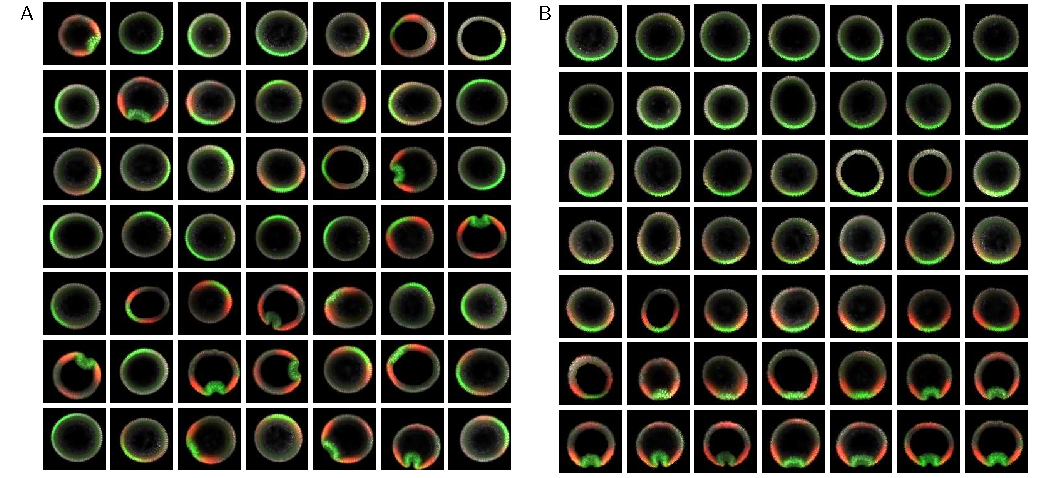
\includegraphics{fig3}
\caption{{\xfigtextfontit Drosophila} embryos during cellularization. {\xfigtextfontit (A)} Images of embryos collected during cellularization. Each image is of a different embryo arrested at a different developmental time, and in a different rotational and translational orientation. {\xfigtextfontit (B)} Images from {\xfigtextfontit A}, now registered and ordered using vector diffusion maps. The images are ordered from left to right and from top to bottom, so that the first image appears in the top left position of the array, and the last image appears in the bottom right position. The dorsal side of each embryo now appears at the top of each image, and the ventral side appears at the bottom.}
\customlabel{fig:data1}{3}
\customlabel{subfig:raw_data1}{\ref{fig:data1}{\it A}}
\customlabel{subfig:ordered_data1}{\ref{fig:data1}{\it B}}
\customlabel{subfig:averaged_data1}{\ref{fig:data1}{\it C}}
\end{figure*}

\subsection{Images of embryos during cellularization}

As a first illustration of using vector diffusion maps to temporally order and register images, we analyze a data set where the correct registration and temporal order is known {\it a priori}.
%
This data set is obtained by fluorescent imaging of {\it Drosophila} embryos during the third hour after fertilization.
%
By this stage of development, sequential divisions of the fertilized egg have generated a system where most of the nuclei are arranged in a monolayer under the common plasma membrane \cite{foe1983studies}.
%
\fig~\ref{subfig:raw_data1} shows optical cross-sections of each embryo, with nuclei (gray in the figure) labeled by DAPI, a DNA stain.
%
During the third hour of development, this arrangement of nuclei is patterned by the concentration profiles of chemical signals that control cell differentiation.
%
One of these signals is provided by the nuclear localization of the transcription factor Dorsal (Dl, green in the figure), which subdivides the early embryo into the territories that give rise to the muscle, nerve, and skin tissues.
%
Another signal is provided by the phosphorylated form of the extracellular signal regulated kinase (dpERK, red in the figure), an enzyme that specifies a subset of neuronal cells.
%


%%%YGK say a simple thing in the caption about Dorsal-Ventral

Previous studies established that throughout the third hour of development, the nuclear localization of Dl is unimodal and peaked at the ventral side of the embryo (reviewed in \cite{rushlow2012temporal}).
%
The spatiotemporal pattern of dpERK is more complex: dpERK is first detected in two lateral stripes, which increase in intensity towards the end of the third hour of development \cite{lim2013kinetics}.
%
This bimodal pattern is then augmented by a peak at the dorsal side of the embryo.
%
Both of these features become readily apparent when images are registered and ordered using vector diffusion maps (see \fig~\ref{subfig:ordered_data1}): the peak of nuclear Dl is consistent throughout the images and the intensity of the dpERK signal in the lateral regions of the embryo increases monotonically across the data set.
%

For this data set, the quality of the temporal ordering provided by vector diffusion maps can be assessed by comparing with the ordering obtained through an independent approach.
%
During the third hour of development, the embryo cellularizes: in this process, nuclei located under a common plasma membrane are enclosed by lateral membranes which grow inward, separating the nuclei into individual cells.
%
The highly reproducible kinetics of lateral membrane growth can be used to estimate the age of each embryo to within 2--3 minutes \cite{figard2013plasma} (see \fig~\ref{fig:membrane_curve}).
%
The Spearman rank correlation coefficient between the orderings obtained based on the progress of cellularization and vector diffusion maps is 0.91, indicating that vector diffusion maps can accurately recover the temporal order.
%
Thus, we have validated a dimensionality reduction approach to temporal ordering and registration on a data set where image orientation and ordering can be assessed independently.

%Although the first vector diffusion maps coordinate accurately captures the developmental dynamics, there are other sources of variability within this data set that could also be extracted using these techniques.
%
%An obvious one is variability due to size; here, the size variation is relatively small relative to the developmental changes and does not significantly obstruct the reconstruction of the temporal order.
%
%However, in other applications where the size variation is significant %or the developmental dynamics are more subtle, it may be important to %factor out size or {\it scaling} symmetries.
%%%
%%%YGK   for teh "additional components" - don't have in the same sentence - say it somewhere else.... INCLUDE IT (maybe in the mutants)


%Furthermore, the dynamics uncovered by vector diffusion maps is relatively simple, which suggests that a simpler approach could have been used to order the data.
%
%Indeed, a principal component analysis (PCA) of registered data reveals that data can be accurately ordered by projecting each image onto the first PCA mode.

\subsection{Images of gastrulating embryos}

%As the images in Figure~\ref{fig:data1} are relatively simple, other techniques could have been used to temporally order them.
%
Because the dynamics of the data set shown in \fig~\ref{fig:data1} are relatively simple, effectively consisting of a single mode (the two dpERK peaks) growing in time, established techniques such as principal component analysis (PCA) \cite{shlens2005tutorial} would uncover most of the meaningful structure in the data, and projection onto the first principal component would be sufficient to order the data in time (see \fig~\ref{fig:PCA_data1}).
%
However, developmental dynamics are often significantly more complex, and nonlinear dimensionality reduction techniques are required to extract meaningful structure.
%
\fig~\ref{subfig:raw_data2} shows a richer data set of $108$ images of {\it Drosophila} embryos.
%
These images cover a thirty minute time interval and span late cellularization through gastrulation, when the two-dimensional sheet of newly formed cells begins to deform into three-dimensional structures which will form the future organs \cite{leptin2005gastrulation}.
%
As before, each image is an optical cross-section of a vertically oriented embryo fixed at a different developmental time.
%
The nuclei (gray) are again labeled with a DNA marker.
%
However, during this developmental time period, the nuclei are no longer uniformly arranged around the periphery of the embryo.
%
Instead of Dl, which is difficult to visualize at this point, embryos were stained with the antibody that recognizes Twist (Twi, shown in green), a transcription factor that is activated by high levels of Dl, specifying the cells of the future muscle tissue.
%
dpERK is again shown in red.

%
During this time window the ventral furrow is formed, where the ventral side buckles towards the center of the embryo, bringing in the future muscle cells.
%
dpERK appears as two lateral peaks at the ventral side of the embryo.
%
These two peaks merge together during invagination, eventually forming (together with Twi) a characteristic ``omega'' shape.
%
Germband extension then causes cells from the ventral side to move towards the posterior pole of the embryo, and then wrap around to the dorsal side \cite{leptin2005gastrulation}.
%
At the end of this process, cells which were originally on the ventral and posterior side of the embryo find themselves on the dorsal side, causing similar ``omega'' shaped patterns to arise on the dorsal side; these patterns are most readily seen in the last image of \fig~\ref{subfig:averaged_data2}.

\begin{figure*}[t]
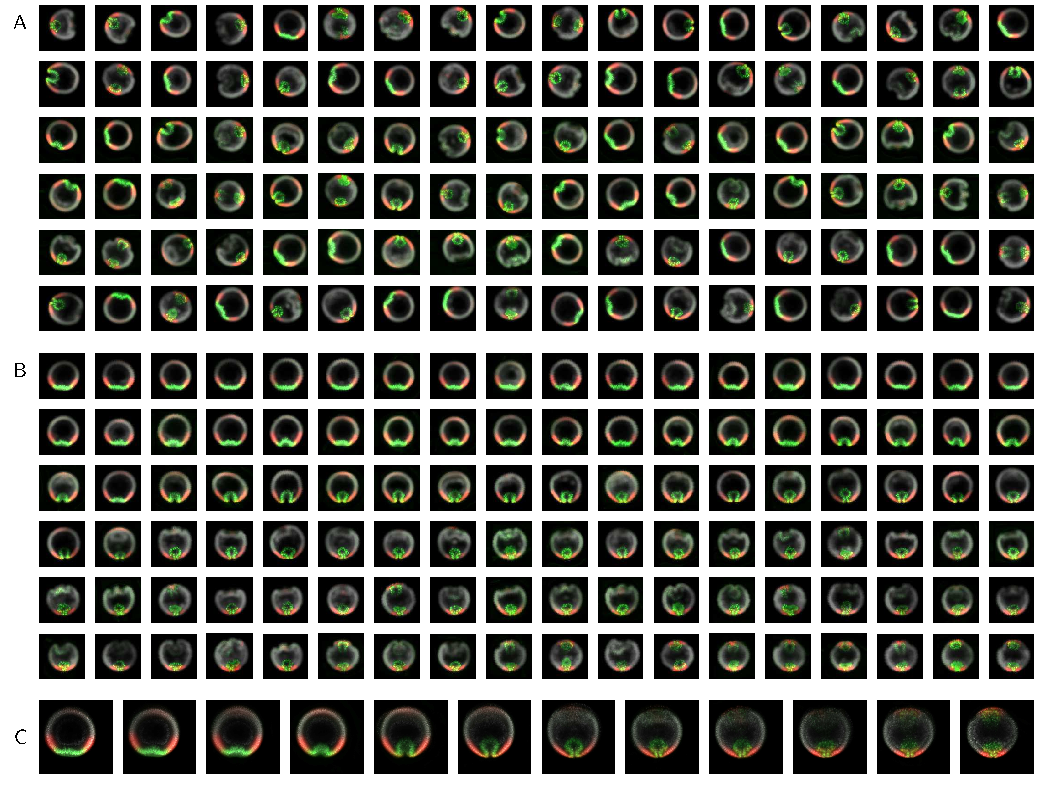
\includegraphics{fig4}
\caption{{\xfigtextfontit Drosophila} embryos during gastrulation. {\xfigtextfontit (A)} Images of gastrulating embryos. Each image is of a different embryo arrested at a different developmental time, and in a different translation and rotational orientation. {\xfigtextfontit (B)} Data from {\xfigtextfontit A}, registered and ordered using vector diffusion maps. The images are ordered from left to right and from top to bottom, so that the first image appears in the top left position of the array, and the last image appears in the bottom right position. {\xfigtextfontit (C)} A representative ``developmental path'' from local averaging of the images. Each image is a (Gaussian-weighted) average of the images in {\xfigtextfontit B}. }
\customlabel{fig:data2}{4}
\customlabel{subfig:raw_data2}{\ref{fig:data2}{\it A}}
\customlabel{subfig:ordered_data2}{\ref{fig:data2}{\it B}}
\customlabel{subfig:averaged_data2}{\ref{fig:data2}{\it C}}
\end{figure*}


Visually, the dynamics in this data set are much more complicated, and only 22\% of the variability in the images is captured by the first principal component.
%
Simple time-ordering based on this linear projection is therefore not possible (see \fig~\ref{fig:PCA_data2}).
%
%Even when projecting on several leading principal components (see SI), a nonlinear approach, such as vector diffusion maps, is required to temporally order the data.
%
\fig~\ref{subfig:ordered_data2} shows the images registered and ordered using vector diffusion maps \cite{singer2012vector}, 
and visual inspection confirms this ordering is consistent with the known developmental dynamics outlined above.
%
However, assimilating the dynamics even from this concatenation of images is difficult for two reasons, even after registration and ordering.
%
First, the sheer number of images makes visual processing of the entire data set nontrivial;
and second, the ordered data is not entirely smooth due to inter-embryo variability.
%
To highlight the developmental dynamics revealed by vector diffusion maps, we applied a Gaussian filter to the trajectory of registered and ordered images to obtain an averaged developmental path (see also \cite{kemelmacher2011exploring}).  
%
Sequential snapshots of this averaged trajectory, shown in \fig~\ref{subfig:averaged_data2}, serve as a summary of the stereotypic developmental dynamics reconstructed from cross-sectional data.
%
Thus, vector diffusion maps can accomplish the image registration and ordering tasks presented in the caricature in \fig~\ref{fig:fish}, even in the absence of information about image landmarks (e.g., fins) and without {\it a priori} knowledge of developmental dynamics (e.g., correlation of age with body size).



\subsection{Additional variability: identifying distinct developmental trajectories}

When time is the main source of variability, we have shown that vector diffusion maps can recover developmental progression from cross-sectional data.
%
However, vector diffusion maps can also provide an organization of data which contains multiple sources of variability.
%
To illustrate this point, we collected a data set consisting of $42$ embryos undergoing cellularization during the third hour of development (see \fig~\ref{fig:raw_data3}).
%
Half of the embryos are wild type, and half of the embryos are mutants where dpERK is expressed in one broad peak at the ventral side.
%
Again, each image is an optical cross-section of an embryo fixed at a different developmental time, and the embryos have been stained for nuclei (gray), Dl (green), and dpERK (red).
%
We expect two sources of variability in this data set: differences due to developmental time, and differences between mutant and wild type dynamics.




We computed the vector diffusion maps embedding for our data, and the eigenvalue distribution (see \fig~\ref{fig:eigenvalues}) indicates that two coordinates may be required for a meaningful description of the data. 
%
\fig~\ref{subfig:projection_data3} shows the data projected onto the first two vector diffusion maps coordinates; each point in this projection corresponds to one image in our data set.
%%%
%%%YGK we need something about dmap eignvalues and how many are not harmonics
%
Two distinct branches appear to emerge in this two-dimensional embedding space.

\begin{figure}[h]
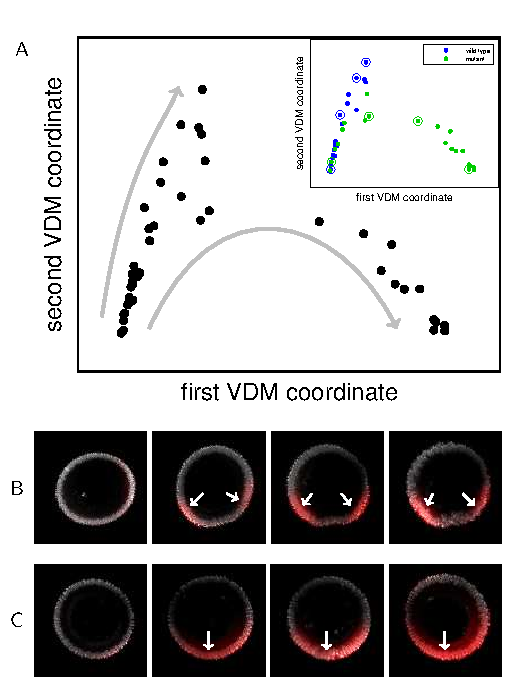
\includegraphics{fig5_2}
%\caption{Wild type and mutant {\xfigtextfontit Drosophila} embryos.  {\xfigtextfontit(A)} Data collected from wild type and mutant embryos (original data set is shown in \fig~\ref{fig:raw_data3}), projected onto the first two vector diffusion maps coordinates. {\xfigtextfontit (B)} The data in {\xfigtextfontit A}, now colored by genotype. The two branches separate mutant and wild type samples, and the direction of the developmental trajectories are indicated by arrows. {\xfigtextfontit (C)} dpERK signal at select wild type points in {\xfigtextfontit B} (denoted by circles). The two dpERK peaks which arise during development are indicated by arrows. {\xfigtextfontit (C)} dpERK signal at select mutant points in {\xfigtextfontit B} (denoted by circles). The single dpERK peak is indicated by an arrow. }
\caption{Wild type and mutant {\xfigtextfontit Drosophila} embryos.  {\xfigtextfontit(A)} Data collected from wild type and mutant embryos (original data set is shown in \fig~\ref{fig:raw_data3}), projected onto the first two vector diffusion maps coordinates. The direction of the developmental trajectories are indicated by arrows. (Inset) The projected data, now colored by genotype. The two branches separate mutant and wild type samples. {\xfigtextfontit (B)} dpERK signal at select points along the wild type trajectory in {\xfigtextfontit A} (denoted by circles in the inset). The two dpERK peaks which arise during development are indicated by arrows. {\xfigtextfontit (C)} dpERK signal at select points along the mutant trajectory in {\xfigtextfontit A} (denoted by circles in the inset). The single dpERK peak is indicated by an arrow. }
\customlabel{fig:data3}{5}
\customlabel{subfig:projection_data3}{\ref{fig:data3}{\it A}}
%\customlabel{subfig:projection_colored_data3}{\ref{fig:data3}{\it B}}
\customlabel{subfig:average_wt_data3}{\ref{fig:data3}{\it B}}
\customlabel{subfig:average_mut_data3}{\ref{fig:data3}{\it C}}
\end{figure}

The inset of \fig~\ref{subfig:projection_data3} shows the two-dimensional projection, with the data points colored to indicate whether they come from the wild type or mutant.
%
Clearly, the two branches in the embedding help distinguish wild type and mutant embryos.
%
Selected images along the wild type and mutant trajectories are shown in \fig~\ref{subfig:average_wt_data3} and \fig~\ref{subfig:average_mut_data3}, respectively.
%
The portion of the embedding where the two genotypes are intermixed (lower-right region of the plot) contains embryos who are early in their developmental trajectory, where there is little dpERK signaling and the two groups of embryos are indistinguishable. 
%
When the two paths diverge, the wild type data develops two distinct peaks, whereas the mutant data develops a single peak.
%
Therefore, vector diffusion maps can also help distinguish different expression patterns and developmental trajectories.




\section{Discussion}

We presented a unified approach to temporal ordering and registration of images in cross-sectional studies of developmental dynamics. 
%
To the best of our knowledge, algorithmic approaches to these two tasks have been explored largely independently of each other. 
%
In particular, temporal ordering of imaging data sets was done with a significant amount of human supervision and using registered images as a starting point \cite{yuan2014automated, surkova2008characterization}.  
%
In parallel, ordering of large-scale cross-sectional data was done in the context of molecular profiling studies, in which data are vectors describing the amounts of different chemical species, such as mRNA abundances \cite{anavy2014blind, trapnell2014dynamics, gupta2008extracting}. 
%
Automated temporal ordering of such data sets was accomplished by first projecting the data on a low-dimensional subspace spanned by the leading principal or independent components, and then solving a traveling salesman problem or constructing a minimum spanning tree on the projected data to order multiple snapshots. 
%
The approach presented here is different because it addresses image registration and ordering in a single step and orders the data without first projecting them on a low-dimensional subspace. 
%
The task of image registration has also been widely studied \cite{zitova2003image}, for applications such as face recognition \cite{rowley1998rotation}, medical image registration \cite{hajnal2010medical}, and texture classification \cite{greenspan1994rotation}.
%
In contrast to most of the existing approaches to image registration which rely on the knowledge about some landmarks in the data \cite{ian1998statistical} (such as the eyes in face recognition applications \cite{zhao2003face}), algorithms based on angular synchronization (such as vector diffusion maps) can register images even in the absence of such information. 
%TODO: look at Eisen Cell paper about registration

We used the technique to analyze three different experimental data sets, collected specifically for this study. 
%
In the first example, correct orientation and temporal order of images was known {\it a priori}, providing a test case for the algorithm in which both of these features were accurately recovered. 
%
For this particular data set, a simpler approach would have sufficed. 
%
Indeed, because of the relative simplicity of developmental dynamics (monotonic increase in the amplitude of a localized signaling pattern and relatively small tissue deformation), temporal order could have been inferred by projection of registered images on the first principal component of the data set (see \fig~\ref{fig:PCA_data1}). 
%
This approach was clearly not sufficient for the second data set (see \fig~\ref{fig:PCA_data2}), collected from embryos during the time window where both the tissue morphology and signaling patterns are rapidly changing.  
%
Vector diffusion maps could readily extract a nontrivial spatiotemporal trajectory. 
%
Finally, the algorithm was applied to a heterogeneous data set, composed of images from embryos of different genotypes. 
%
In this case, low-dimensional projection of registered data revealed distinct paths that correlated with the developmental trajectories of the mutant and wild type populations. 

Previously, angular synchronization and vector diffusion maps have been used to reconstruct molecular shapes from cryo-electron microscopy imaging data \cite{singer2012vector, singer2011three}. 
%
Because of the high levels of instrument noise in these images, thousands of images were needed for successful shape reconstruction. 
%
Based on our work, we expect that much smaller data sets may be sufficient for successful reconstruction of developmental trajectories, providing the first step in systems level studies of embryogenesis. 
%
In the future, functional data analysis tools can be used for the quantitative estimation of both the average trajectory and its variability \cite{silverman2005functional}.  
%
One can also test which physical variable, among a set of candidate variables, is most correlated with the uncovered vector diffusion maps coordinate to gain insight into which physical quantities change across the developmental trajectory (e.g., total intensity of one signal, roundness of the embryo).
%
Here, we have used vector diffusion maps to register the images with respect to translations and rotations; however, it is conceivable that one could factor out other sources of variability, such as reflections \cite{singer2012vector, goemans1995improved} or dilations, in the images.
%
One might even envision automated analysis of embryos imaged in arbitrary three-dimensional orientations, in the spirit of cryo-EM image analysis.
%
We believe that algorithms based on image features which are insensitive to small deformations, such as the scattering transform \cite{mallat2012group}, are especially promising.
%
Another important application is related to the joint analysis of data sets provided by different imaging approaches, such as merging live imaging data of tissue morphogenesis with snapshots of cell signaling and gene expression from fixed embryos \cite{krzic2012multiview, ichikawa2014live, rubel2010coupling}. 
%
Given the rapidly increasing volumes of imaging data from studies of multiple developmental systems, we expect that dimensionality reduction approaches discussed in this work will be increasingly useful for biologists and motivate future applications and algorithmic advances. 
  

%% == end of paper:

%% Optional Materials and Methods Section
%% The Materials and Methods section header will be added automatically.

%% Enter any subheads and the Materials and Methods text below.


\begin{materials}

\section{Fly strain and whole-mount immunostaining}
%
Oregon-R (OreR) and spaghetti squash (Sqh)-GFP were used as wild type strains. 
%
{\it Sna\textsuperscript{\it IIG05}/Cyo hb-lacZ} flies were used to study embryos with one peak of dpERK expression.  
%
Embryos were collected and fixed at 22$^\circ$C. 
%
Monoclonal rabbit anti-dpERK (1:100, Cell signaling), mouse anti-Dorsal (1:100, Developmental Studies Hybridoma Bank), rat anti-Twist (1:500, a gift from Eric Wieschaus), and mouse anti-beta-galactosidase (1:500, DSHB) were used to stain proteins of interest. DAPI (1:10,000, Vector Laboratories) was used to visualize nuclei, and Alexa Fluors (1:500, Invitrogen) were used as secondary antibodies. 

\section{Microscopy}
%
Nikon A1-RS scanning confocal microscope, and the Nikon 60X Plan-Apo oil objective was used to image embryos. Embryos were collected, stained, and imaged together under the same microscope setting. End-on imaging was performed by using the microfluidics device described previously. Images were collected at the focal plane $\sim$90~$\mathrm{\mu m}$ from the posterior pole of an embryo (see \fig~\ref{fig:DV_view}). 

\section{Development time during cellularization} 
%
The progression of membrane invagination during cellularization was used to assign time point to each embryo in the third hour of development. Time-lapse imaging of Sqh-GFP embryo was used to generate correlation curve between the membrane ingression length and the developmental time (n=7) (\fig~\ref{fig:membrane_curve}B). The rate at which membrane invaginates was highly reproducible from embryo to embryo. In the experiments with fixed embryos, we measured the membrane length by co-staining embryos with a membrane marker (Sqh-GFP) or by taking phase-contrast images (\fig~\ref{fig:membrane_curve}A). We used the correlation curve to assign each embryo to a time window of 2--3~minutes. 

\end{materials}


%% Optional Appendix or Appendices
%% \appendix Appendix text...
%% or, for appendix with title, use square brackets:
%% \appendix[Appendix Title]


\begin{acknowledgments}
The authors thank Adam Finkelstein,  Thomas Funkhouser, and John Storey for helpful discussions. 
%
C.J.D. was supported by the Department of Energy Computational Science Graduate Fellowship (CSGF), grant number DE-FG02-97ER25308.
%
B.L. and S.Y.S. were supported by the National Institutes of Health Grant R01GM086537. 
%
T.J.L. and H.L. were supported by the National Science Foundation Grant Emerging Frontiers in Research and Innovation (EFRI) 1136913.
%
I.G.K. was supported by the National Science Foundation (CS\&E program).
\end{acknowledgments}

%% PNAS does not support submission of supporting .tex files such as BibTeX.
%% Instead all references must be included in the article .tex document.
%% If you currently use BibTeX, your bibliography is formed because the
%% command \verb+\bibliography{}+ brings the <filename>.bbl file into your
%% .tex document. To conform to PNAS requirements, copy the reference listings
%% from your .bbl file and add them to the article .tex file, using the
%% bibliography environment described above.

%%  Contact pnas@nas.edu if you need assistance with your
%%  bibliography.

% Sample bibliography item in PNAS format:
%% \bibitem{in-text reference} comma-separated author names up to 5,
%% for more than 5 authors use first author last name et al. (year published)
%% article title  {\it Journal Name} volume #: start page-end page.
%% ie,
% \bibitem{Neuhaus} Neuhaus J-M, Sitcher L, Meins F, Jr, Boller T (1991)
% A short C-terminal sequence is necessary and sufficient for the
% targeting of chitinases to the plant vacuole.
% {\it Proc Natl Acad Sci USA} 88:10362-10366.


%% Enter the largest bibliography number in the facing curly brackets
%% following \begin{thebibliography}

%\bibliographystyle{pnas2}
%\bibliography{background_reading/references,../../references/references}

\begin{thebibliography}{10}

\bibitem{diggle2002analysis}
Diggle P, Heagerty P, Liang K~Y, Zeger S (2002) \textit{Analysis of
  longitudinal data} (Oxford University Press).

\bibitem{roelens2013live}
Roelens B, Chanes J~D~L~H, Dostatni N (2013) Live imaging of bicoid-dependent
  transcription in \textit{{D}rosophila} embryos. \textit{Curr Biol}
  23:1--5.

\bibitem{keller2013imaging}
Keller P~J (2013) Imaging morphogenesis: technological advances and biological
  insights. \textit{Science} 340(6137).

\bibitem{jaeger2004dynamic}
Jaeger J, Surkova S, Blagov M, Janssens H, Kosman D, \textit{et~al.} (2004)
  Dynamic control of positional information in the early \textit{{D}rosophila}
  embryo. \textit{Nature} 430(6997):368--371.

\bibitem{fowlkes2008quantitative}
Fowlkes C~C, Hendriks C~L~L, Ker{\"a}nen S~V, Weber G~H, R{\"u}bel O,
  \textit{et~al.} (2008) A quantitative spatiotemporal atlas of gene expression
  in the \textit{{D}rosophila} blastoderm. \textit{Cell} 133(2):364--374.

\bibitem{ng2012large}
Ng L~L, Sunkin S~M, Feng D, Lau C, Dang C, \textit{et~al.} (2012) Large-scale
  neuroinformatics for in situ hybridization data in the mouse brain.
  \textit{Int Rev Neurobiol} 104:159--182.

\bibitem{richardson2014emage}
Richardson L, Stevenson P, Venkataraman S, Yang Y, Burton N, \textit{et~al.}
  (2014) Emage: Electronic mouse atlas of gene expression, \textit{Mouse
  Molecular Embryology} (Springer), pp. 61--79.

\bibitem{castro2009automatic}
Castro C, Luengo-Oroz M, Desnoulez S, Duloquin L, Fernandez-de Manuel L,
  \textit{et~al.} (2009) An automatic quantification and registration strategy
  to create a gene expression atlas of zebrafish embryogenesis,
  \textit{Conf Proc IEEE Eng Med Biol Soc}, pp. 1469--1472.

\bibitem{zitova2003image}
Zitova B, Flusser J (2003) Image registration methods: a survey. \textit{Image Vis Comput} 21(11):977--1000.

\bibitem{rowley1998rotation}
Rowley H~A, Baluja S, Kanade T (1998) Rotation invariant neural network-based
  face detection, \textit{Computer Vision and Pattern Recognition, 1998.
  Proceedings. 1998 IEEE Computer Society Conference on} (IEEE), pp. 38--44.

\bibitem{hajnal2010medical}
Hajnal J~V, Hill D~L (2010) \textit{Medical image registration} (CRC press).

\bibitem{greenspan1994rotation}
Greenspan H, Belongie S, Goodman R, Perona P (1994) Rotation invariant texture
  recognition using a steerable pyramid, \textit{Pattern Recognition, 1994.
  Vol. 2-Conference B: Computer Vision \& Image Processing., Proceedings of the
  12th IAPR International. Conference on} (IEEE), volume~2, pp. 162--167.

\bibitem{zhao2003face}
Zhao W, Chellappa R, Phillips P~J, Rosenfeld A (2003) Face recognition: A
  literature survey. \textit{ACM Computing Surveys (CSUR)} 35(4):399--458.

\bibitem{singer2012vector}
Singer A, Wu H~T (2012) Vector diffusion maps and the connection laplacian.
  \textit{Commun Pure Appl Math} 65(8):1067--1144.

\bibitem{Belkin2003}
Belkin M, Niyogi P (2003) Laplacian eigenmaps for dimensionality reduction and
  data representation. \textit{Neural Comput} 15:1373--1396.

\bibitem{coifman2005geometric}
Coifman R~R, Lafon S, Lee A~B, Maggioni M, Nadler B, \textit{et~al.} (2005)
  Geometric diffusions as a tool for harmonic analysis and structure definition
  of data: Diffusion maps. \textit{Proc Natl Acad Sci USA} 102(21):7426--7431.

\bibitem{coifman2006geometric}
Coifman R~R, Lafon S (2006) Geometric harmonics: a novel tool for multiscale
  out-of-sample extension of empirical functions. \textit{Appl Comput Harmon Anal} 21(1):31--52.

\bibitem{tenenbaum2000global}
Tenenbaum J~B, De~Silva V, Langford J~C (2000) A global geometric framework for
  nonlinear dimensionality reduction. \textit{Science} 290(5500):2319--2323.

\bibitem{roweis2000nonlinear}
Roweis S~T, Saul L~K (2000) Nonlinear dimensionality reduction by locally
  linear embedding. \textit{Science} 290(5500):2323--2326.

\bibitem{jaeger2012drosophila}
Jaeger J, Manu, Reinitz J (2012) \textit{{D}rosophila} blastoderm patterning.
  \textit{Curr Opin Genet Dev} 22(6):533 -- 541, genetics of system biology.

\bibitem{singer2011angular}
Singer A (2011) Angular synchronization by eigenvectors and semidefinite
  programming. \textit{Appl Comput Harmon Anal}
  30(1):20--36.

\bibitem{ahuja2007template}
Ahuja S, Kevrekidis I~G, Rowley C~W (2007) Template-based stabilization of
  relative equilibria in systems with continuous symmetry. \textit{Journal of
  Nonlinear Science} 17(2):109--143.

\bibitem{ian1998statistical}
Dryden I~L, Mardia K (1998) \textit{Statistical shape analysis}, Wiley series
  in probability and statistics: Probability and statistics (J. Wiley).

\bibitem{foe1983studies}
Foe V~E, Alberts B~M (1983) Studies of nuclear and cytoplasmic behaviour during
  the five mitotic cycles that precede gastrulation in \textit{{D}rosophila}
  embryogenesis. \textit{J Cell Sci} 61(1):31--70.

\bibitem{rushlow2012temporal}
Rushlow C~A, Shvartsman S~Y (2012) Temporal dynamics, spatial range, and
  transcriptional interpretation of the dorsal morphogen gradient.
  \textit{Curr Opin Genet Dev} 22(6):542--546.

\bibitem{lim2013kinetics}
Lim B, Samper N, Lu H, Rushlow C, Jim{\'e}nez G, \textit{et~al.} (2013)
  Kinetics of gene derepression by erk signaling. \textit{Proc Natl Acad Sci USA} 110(25):10330--10335.

\bibitem{figard2013plasma}
Figard L, Xu H, Garcia H~G, Golding I, Sokac A~M (2013) The plasma membrane
  flattens out to fuel cell-surface growth during \textit{{D}rosophila}
  cellularization. \textit{Dev Cell} 27(6):648--655.

\bibitem{shlens2005tutorial}
Shlens J (2005) A tutorial on principal component analysis. \textit{Systems
  Neurobiology Laboratory, University of California at San Diego} .

\bibitem{leptin2005gastrulation}
Leptin M (2005) Gastrulation movements: the logic and the nuts and bolts.
  \textit{Dev Cell} 8(3):305--320.

\bibitem{kemelmacher2011exploring}
Kemelmacher-Shlizerman I, Shechtman E, Garg R, Seit, S~M (2011)
Exploring photobios. \textit{ACM Transactions on Graphics (TOG)} 30(4):61.

\bibitem{yuan2014automated}
Yuan L, Pan C, Ji S, McCutchan M, Zhou Z~H, \textit{et~al.} (2014) Automated
  annotation of developmental stages of \textit{{D}rosophila} embryos in images
  containing spatial patterns of expression. \textit{Bioinformatics}
  30(2):266--273.

\bibitem{surkova2008characterization}
Surkova S, Kosman D, Kozlov K, Myasnikova E, Samsonova A~A, \textit{et~al.}
  (2008) Characterization of the \textit{{D}rosophila} segment determination
  morphome. \textit{Dev Biol} 313(2):844--862.

\bibitem{anavy2014blind}
Anavy L, Levin M, Khair S, Nakanishi N, Fernandez-Valverde S~L, \textit{et~al.}
  (2014) Blind ordering of large-scale transcriptomic developmental
  timecourses. \textit{Development} 141(5):1161--1166.

\bibitem{trapnell2014dynamics}
Trapnell C, Cacchiarelli D, Grimsby J, Pokharel P, Li S, \textit{et~al.} (2014)
  The dynamics and regulators of cell fate decisions are revealed by
  pseudotemporal ordering of single cells. \textit{Nat Biotechnol} 32(4):381--386.

\bibitem{gupta2008extracting}
Gupta A, Bar-Joseph Z (2008) Extracting dynamics from static cancer expression
  data. \textit{IEEE/ACM Trans Comput Biol Bioinform} 5(2):172--182.

\bibitem{singer2011three}
Singer A, Shkolnisky Y (2011) Three-dimensional structure determination from
  common lines in cryo-em by eigenvectors and semidefinite programming.
  \textit{SIAM J Imaging Sci} 4(2):543--572.

\bibitem{silverman2005functional}
Ramsay J~O, Silverman B~W (2005) \textit{Functional Data Analysis}, Springer
  Series in Statistics (Springer).

\bibitem{goemans1995improved}
Goemans M~X, Williamson D~P (1995) Improved approximation algorithms for maximum cut and satisfiability problems using semidefinite programming.
\textit{Journal of the ACM} 42(6):1115--1145.

\bibitem{mallat2012group}
Mallat, S (2012) Group invariant scattering. 
\textit{Communications on Pure and Applied Mathematics}
65(10):1331--1398.

\bibitem{krzic2012multiview}
Krzic U, Gunther S, Saunders T~E, Streichan S~J, Hufnagel L (2012) Multiview
  light-sheet microscope for rapid in toto imaging. \textit{Nat Methods}
  9(7):730--733.

\bibitem{ichikawa2014live}
Ichikawa T, Nakazato K, Keller P~J, Kajiura-Kobayashi H, Stelzer E~H,
  \textit{et~al.} (2014) Live imaging and quantitative analysis of gastrulation
  in mouse embryos using light-sheet microscopy and 3d tracking tools.
  \textit{Nat Protoc} 9(3):575--585.

\bibitem{rubel2010coupling}
R{\"u}bel O, Ahern S, Bethel E, Biggin M~D, Childs H, \textit{et~al.} (2010)
  Coupling visualization and data analysis for knowledge discovery from
  multi-dimensional scientific data. \textit{Procedia Comput Sci}
  1(1):1757--1764.

\end{thebibliography}



\end{article}

\end{document}



